%%%%%%%%%%%%%%%%%%%%%%%%%%%%%%%%%%%%%%%%%%%%%%%%%%%%%%%%%%%%%%%%%%%%%%%%%%%%%%
%%
%% This file is part of the ASTERICS Framework. 
%%
%% (C) 2019 Hochschule Augsburg, University of Applied Sciences
%% Efficient Embedded Systems Group
%%
%% Author(s): Thibaut Temkeng <Thibaut.Temkeng@hs-augsburg.de>
%%
%%%%%%%%%%%%%%%%%%%%%%%%%%%%%%%%%%%%%%%%%%%%%%%%%%%%%%%%%%%%%%%%%%%%%%%%%%%%%%

	
\section{Graphical User Interface}\label{ch:06-05-tools-gui}

\secauthor{Thibaut Temkeng}

\infobox{The \asterics-GUI is still in development and not fully tested. See the application and this documentation as in-flux and experimental.}

This chapter introduces and describes the functionality of \asterics-GUI, the graphical user interface (GUI) of \asterics. The GUI is under constant development and its main goal is to speed up the learning curve for \asterics users, even if they have little programming knowledge. In other words, to make the use of the \asterics framework as easy as possible for the end user. The GUI offers the possibility to quickly become familiar with \asterics modules by listing all modules available in \asterics, providing module information such as port, generic, interface, dependencies, the path of the file describing the module, and how the module can be incorporated into an image processing chain. For more information on \asterics modules, see Section \ref{sec:06-05-modullist}. The GUI can also generate a complete functional image processing chain. For this purpose, a wizard is integrated into the GUI that guides the user step by step in the creation of an image processing chain as a Python script. The wizard can help you create your own image processing chain from scratch or create an image processing chain using a template that already exists in \asterics, see Section \ref{sec:06-05-wizard} for more information about the wizard.
	
	\subsubsection*{Prerequisites}
	\begin{itemize}
		\item An \asterics installation. See Section \ref{sec:02-installation}.
		\item Python 3.5 or a higher version.
		\item QT5, version \texttt{5.5} or higher
		\item Pandas. Installation using \textbf{pip install pandas}.
		\item The PyQt5 GUI library. Installation using \textbf{pip install pyqt5}.
	\end{itemize}

	\infobox{Note: On some Linux distributions installation of Python packages may require the use of the command \texttt{pip3} instead of \texttt{pip}. The package \texttt{pip[3]} may also need to be installed.}	
	
	\subsubsection*{Start the GUI}
	\begin{enumerate}
		\item Install the \asterics Framework (see chapter \ref{sec:02-installation}).
		\item Run the command line \texttt{"source settings.sh"} to source the \asterics settings file. The file \texttt{settings.sh} is located in the repository's root folder.
		\item Run the \texttt{"as-gui"} command to start the GUI and you should now have a window like the one shown in \ref{fig:GuiMainView}.
	\end{enumerate}

		\begin{figure}[!ht]
		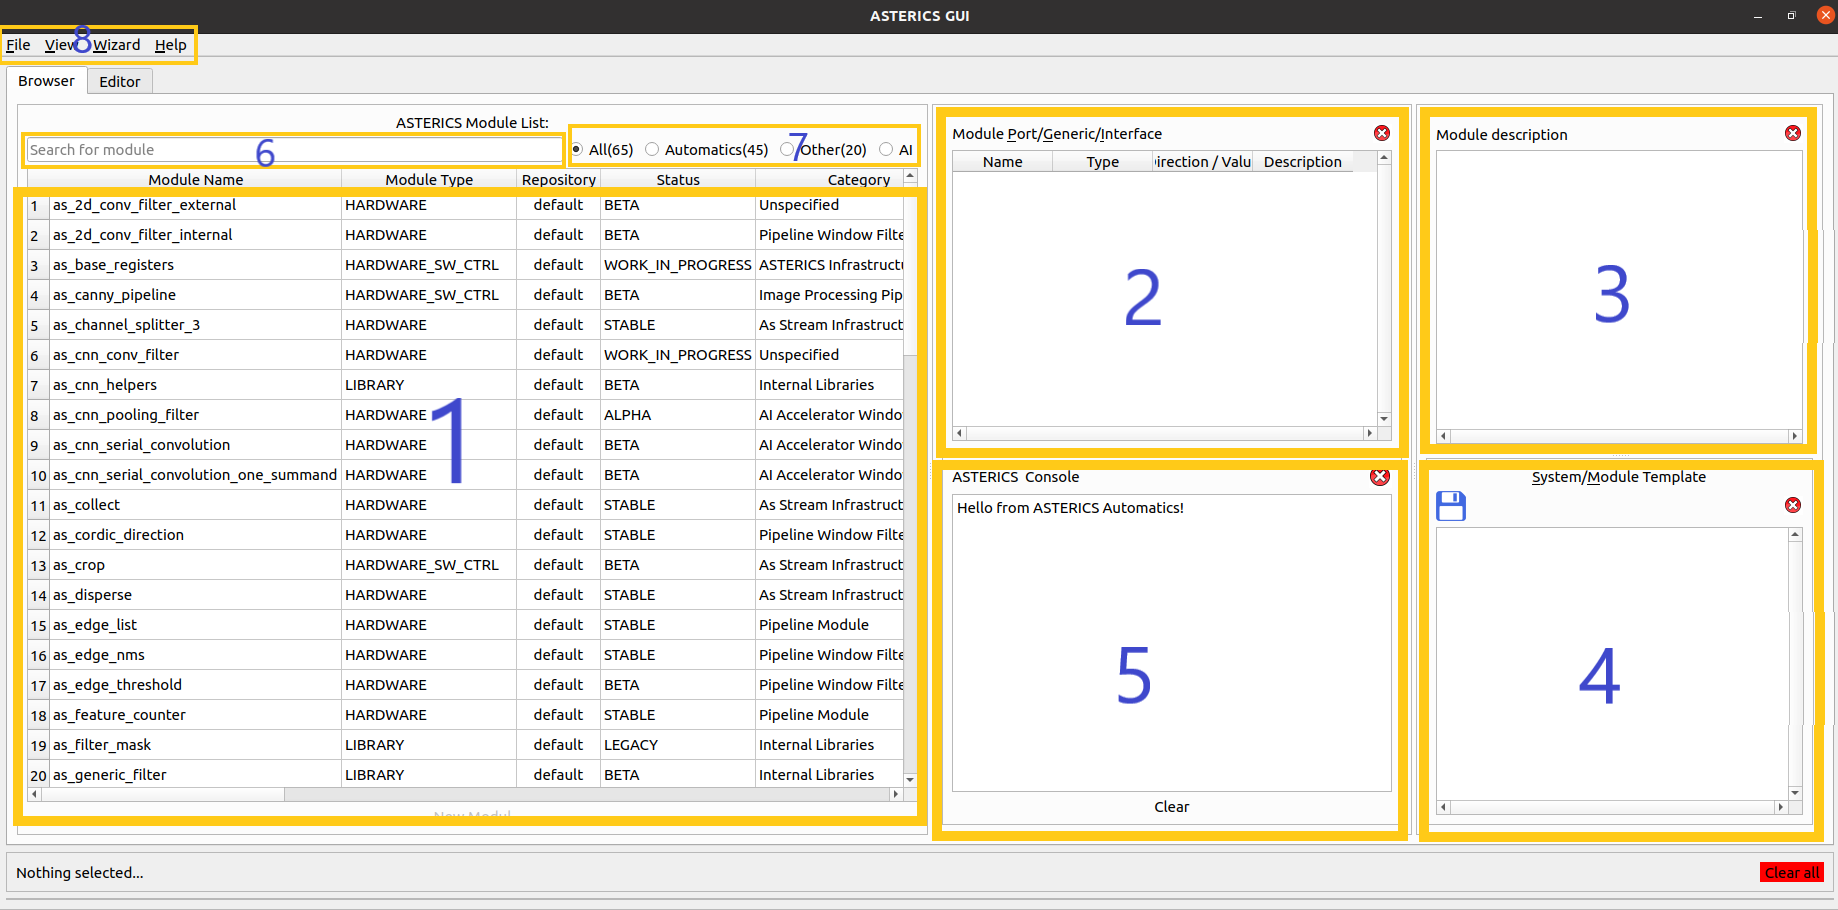
\includegraphics[width=\textwidth]{figs/gui/modulBrowser}
		\caption{GUI main view}
		\label{fig:GuiMainView}
	\end{figure}

	\subsection{Module Browser}
		\label{sec:06-05-modullist}
	This section explains how to use the \asterics-GUI to get details about the image processing modules available in \asterics.
	

	As it can be seen in the figure \ref{fig:GuiMainView}, the main GUI view is divided into smaller views with different goals. In the following, the different functionalities of these subviews will be described:
	\begin{enumerate}
		\item \textbf{Table of \asterics modules list}:\\
			Each row of this table describes an \asterics module and each row contains the following information:
		\begin{itemize}
			\item \lstcinline{Module Name}:\\
				The module name the same as the VHDL entity name.
			\item \lstcinline{Module type}: \\
				Each module has a type that is used to distinguish the modules that can process data e.g. only in hardware or only in software. In the table \ref{tab:06-05-module-type} all module types and the corresponding signification are listed:

			\begin{table}[!ht]
				\centering
				\footnotesize
				\begin{tabular}{|r|l|}
					\hline
					 \textbf{Module type} & \textbf{Signification} \\ \hline
					 UNSPECIFIED & No type specified \\ \hline
					 HARDWARE &Main \asterics hardware processing module \\ \hline
					 SOFTWARE &Main \asterics software processing module \\ \hline
					 LIBRARY& Library sub-module not fur use by the user (automatically inserted) \\ \hline
					 HARDWARE\_SOFTWARE &Main \asterics module processing both in software and hardware \\ \hline
					 HARDWARE\_SW\_CTRL& Main \asterics hardware processing module with a software driver \\ \hline
				\end{tabular}
				\caption{Module Type}
				\label{tab:06-05-module-type}
			\end{table}
			\item \lstcinline{Status}:\\
				From the beginning to the end of the implementation of a module, several steps are required, which are explained in the table \ref{tab:06-05-module-status}: 
		\begin{table}[!ht]
			\centering
			\footnotesize
			\begin{tabular}{|r|l|}
				\hline
				\textbf{Status} & \textbf{Signification} \\ \hline
				UNKNOWN& No state specified.\\ \hline
				 WORK\_IN\_PROGRESS &Code in development.\\ \hline
				 STABLE &In working condition and tested.\\ \hline
				 ALPHA &Code in development, some features work.\\ \hline
				 UNMAINTAINED& No longer maintained, not tested in current code base.\\ \hline
				 LEGACY& In working condition and maintained, but no longer up to date.\\ \hline
				 BETA &Code works, but not tested completely and not necessarily feature complete.\\ \hline
			\end{tabular}
			\caption{Module Status}
			\label{tab:06-05-module-status}
		\end{table}
		\item \lstcinline{Category}:\\
			The module category groups modules by their functionality.
		\item \lstcinline{Documentation}:\\It is currently under development. It is foreseen that this column contains a link that links the Doxygen documentation (to C, VHDL, or Python file) of the module.
		\item \lstcinline{Description}:\\ A rough description of the module.
		\end{itemize}
		\item \textbf{Module Port/Generic/Interface}:\\
			All ports, generics and interfaces of a module are listed here.
		\item \textbf{Modules Description }\\
		Here the module is described in more detail. We get additional information like on which modules the corresponding module depends and the path of the file that contains the implementation of the module.
		\item \textbf{System/Module Template}:\\
		In this view a generated Automatics script is displayed, which can then be saved locally with the button in the upper left corner.
		For something to be displayed in this view, there are two possibilities:
		\begin{enumerate}
			\item Click on a module from the first view.\\
			The generated script here is not a complete Automatics script, it only shows how the module should look like if it would be inserted into an image processing chain, no connection commands are generated.
			\item Click on the \texttt{"generate"} or \texttt{"Finish"} button from the wizard.\\
			The generated script is a complete and functional \automatics script and can therefore be used directly. In most cases, the generated script should be customized before use. 
		\end{enumerate}
		\item \textbf{\asterics Console}:\\
		This view shows the GUI history.
		\item \textbf{Search Bar}:\\
		The search bar facilitates the search for modules.  
		A module can be found by a part of the module name.  It is also useful that the part of the module's name does not have to match the beginning of the module name. For example, if the module \texttt{"as\_canny\_pipeline\_ent"} is searched, the keywords such as \texttt{"can"}, \texttt{"pip"}, \texttt{"ent"} etc can be used to search. Modules can also be searched by category, status or module type. Using the search word \texttt{"BETA"} will only list modules that have the status \texttt{"BETA"}.
		\item \textbf{Filter}:\\
		Not all \asterics modules can be directly introduced into an image processing chain, because they are e.g only sub- or auxiliary modules or also because \automatics cannot automatically include all modules into an image processing chain. With the option button \texttt{"All"} all \asterics modules are displayed, with \texttt{"Automatics"} all modules are listed which \automatics can automatically integrate into an image processing chain and with \texttt{"Other"} all modules not supported by \automatics are listed.
		\item \textbf{Menu Bar}:\\
			The menu bar offers the possibility to control the GUI more easily. The functionality of each menu are described in the following
			\begin{itemize}
				\item \textbf{File}:\\This menu provides two actions:
					\begin{enumerate}
						\item \lstapyinline{Exit}: Close the GUI. The key combination \textit{Ctrl+W} can be used to trigger this action.
						\item \lstapyinline{Add Repository}: It is currently under development. This should allow adding a folder as a new repository to the module library and adding all new modules to the module list. The key combination \textit{Ctrl+N} can be used to trigger this action.
					\end{enumerate}
				\item \textbf{View}: \\This menu provides five actions:
					\begin{enumerate}
						\item \lstapyinline{Template}: This action hides or shows the \textit{System/Module Template} view.
						\item \lstapyinline{Console}: This action hides or shows the \textit{Console} view.
						\item \lstapyinline{Port/Generic/Interface}: This action hides or shows  the \textit{Port/Generic/Interface} view.
						\item \lstapyinline{Modules Description}: This action hides or shows  the \textit{Module Description} view.
						\item \lstcinline{Restore all Views}: This action can be used to restore all views if they were previously closed.
					\end{enumerate}
				\item \textbf{Wizard}:\\This menu provides two actions:
					\begin{enumerate}
						\item \lstcinline{Start}: Start the Wizard. The key combination \textit{Ctrl+O} can be used to trigger this action.
						\item \lstcinline{Close}: Close the Wizard.
					\end{enumerate}
				\item \textbf{Help}: \\It is currently under development. It will allow you get information about \asterics such as the link to the Doxygen documentation of C, VHDL and Python files, new features to come,the contact of people who can help you in case of problems with \asterics and even more.
			\end{itemize}

	\end{enumerate}
	\subsection{Wizard}\label{sec:06-05-wizard}
	This section deals with ways to quickly create simple linear image processing chains. By linear it is meant that all modules in the chain excluding the input and output module get a single input and give a single output.
	There are two ways to create an image processing chain: either build the image processing chain from scratch (see Section \ref{subsub:06-05-new-system}), or use a template available in \asterics as a basis (see Section \ref{subsub:06-05-new-system-based-on-template}).
	To start the wizard, you should press the \texttt{"systems"} button in the 8th view (see the \ref{fig:GuiMainView} figure). A window like in \ref{fig:wizard} should appear. Now you can simply follow the instructions to create your image processing chain.
	\begin{figure}[!ht]
		\centering
		\begin{minipage}{0.45\textwidth}
			\centering
			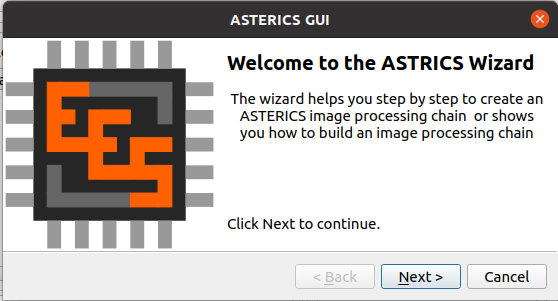
\includegraphics[width=\textwidth]{figs/gui/wizard}
			\caption{Wizard start window}
			\label{fig:wizard}
		\end{minipage} 
		\hfill
		\begin{minipage}{0.45\textwidth}
			\centering
			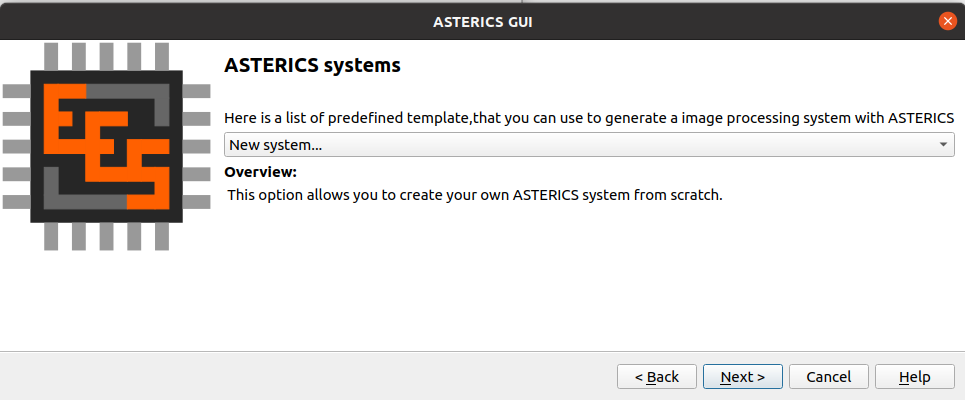
\includegraphics[width=\textwidth,]{figs/gui/list}
			\caption{List of \asterics Systems}

			\label{fig:astericsList}
		\end{minipage}
		
		
	\end{figure}
	\subsubsection{Generate a new System from scratch}\label{subsub:06-05-new-system}
	This section explains how to use the wizard to create a new image processing chain from scratch.
	Exactly how the creation proceeds is shown in the figure \ref{fig:06-05-wizard_input} to \ref{fig:06-05-wizard_connexion} and described in the following steps.
	\begin{figure}[!ht]
		\centering
		\begin{minipage}{0.45\textwidth}
			\centering
			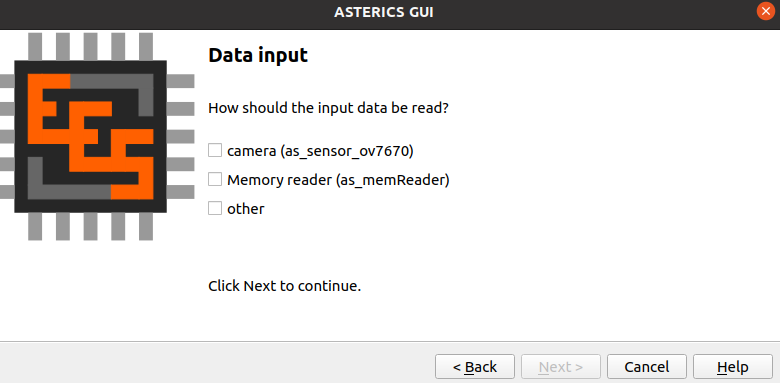
\includegraphics[width=\textwidth]{figs/gui/datainput}
			\caption{Input source}
			\label{fig:06-05-wizard_input}
		\end{minipage} 
		\hfill
		\begin{minipage}{0.45\textwidth}
			\centering
			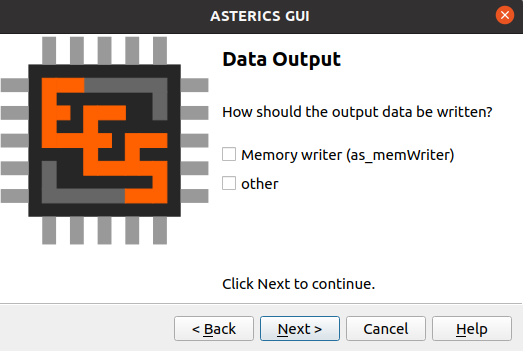
\includegraphics[width=\textwidth,]{figs/gui/dataoutput}
			\caption{Output source}
			\label{fig:06-05-wizard_output}
		\end{minipage}
		\begin{minipage}{0.45\textwidth}
			\centering
			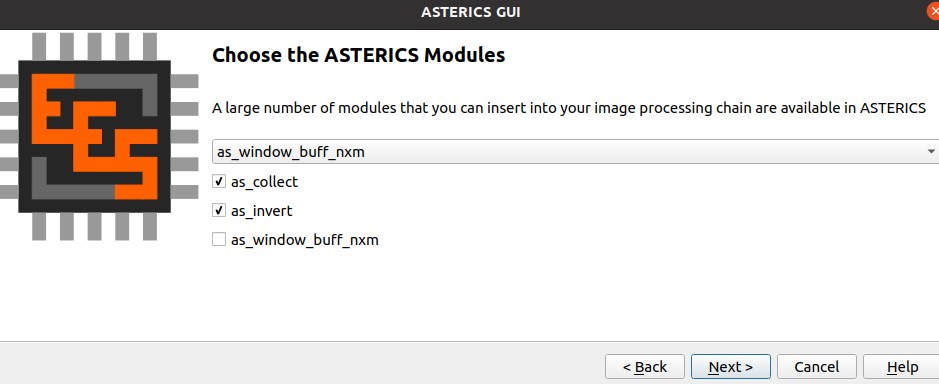
\includegraphics[width=\textwidth]{figs/gui/choose}
			\caption{Choose moduls}
			\label{fig:06-05-wizard_choose}
		\end{minipage} 
		\hfill
		\begin{minipage}{0.45\textwidth}
			\centering
			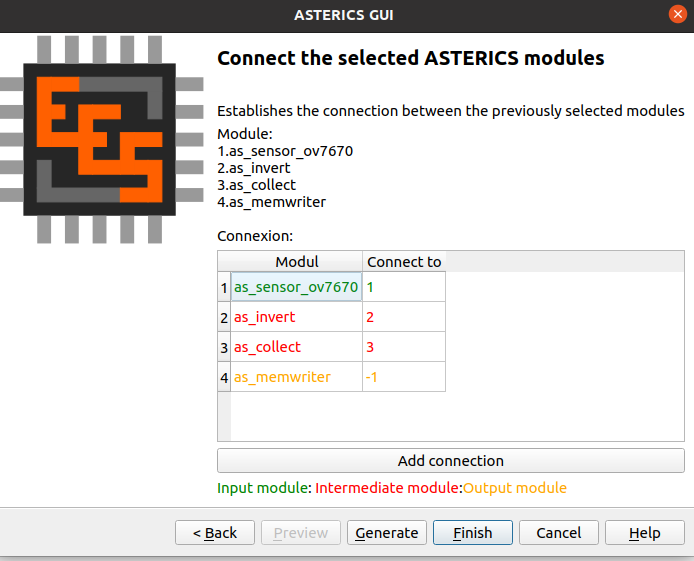
\includegraphics[width=\textwidth,]{figs/gui/connection}
			\caption{Connect moduls}
			\label{fig:06-05-wizard_connexion}
		\end{minipage}
	\end{figure}
	
	\begin{enumerate}
		\item Figure \ref{fig:06-05-wizard_input}: Choose how the input to the image processing chain is to be read. The input can be read directly from the camera, which corresponds to the \texttt{camera(as\_sensor\_ov7670)} option, or read from a file (image or video) from the hard disk, which corresponds to the \texttt{Memory reader (as\_memReader)} option. The latter option \texttt{other} is currently under development and intended for other input sources like USB stick.
		
		\item Figure \ref{fig:06-05-wizard_output}: After the input source has been selected, it should now be selected how the processed input should be written. With the option \texttt{Memory writer (as\_memWriter)} the output is written to memory and the option \texttt{other} is currently under development.
		
		\item Figure \ref{fig:06-05-wizard_choose}: The modules that are to process the input are selected from the list. It must be considered that not all \asterics modules are listed here because Automatics cannot automatically include all modules in an image processing chain or because they have already been used as input modules or output modules. If a selected module is not to be used any more, it must be simply checked off and is not considered in further.
		
		\item Figure \ref{fig:06-05-wizard_connexion}: Now the selected \asterics modules should be connected. In this view, all modules involved in the image processing chain are listed, and then how these modules are connected is shown in a table. In green is the input module (currently only one input module can exist in the chain, so it cannot read data from different input sources into one chain), in red are the intermediate modules (modules that process the input), and in yellow is the output module. The connection between two modules is shown in the column \texttt{"connect to"}. The first row in the table from the figure \ref{fig:06-05-wizard_connexion} means that the input module \texttt{as\_sensor\_ov7670} is directly connected to the module \texttt{as\_invert}. The number in the column  \texttt{"connect to"} must always be added by one to find the corresponding module or row from the table. The number in the \texttt{"connect to"} column are not fixed and can be adjusted. -1 means that the output of the module will not be processed further, the -1 is intended for the output module.  To generate the system, click on the button \texttt{"Generate"} or \texttt{"Finish"}. The generated script is located in the 4th view of the figure \ref{fig:GuiMainView} and can then be customized and saved.See Section \ref{subsub:06-05-generated-script} for further processing of the generated script 
	\end{enumerate}
	\subsubsection{Generate a new System based on Template}\label{subsub:06-05-new-system-based-on-template}
	This section explains how to use the Wizard to create a new computer vision system based on a template available in \asterics. The \asterics framework provides demonstration systems to facilitate familiarization with the concepts of the framework and its modules. The demo systems are already functional and can be used as a template for creating other systems.
	\begin{figure}[!ht]
		\centering
		\begin{minipage}{0.47\textwidth}
			\centering
			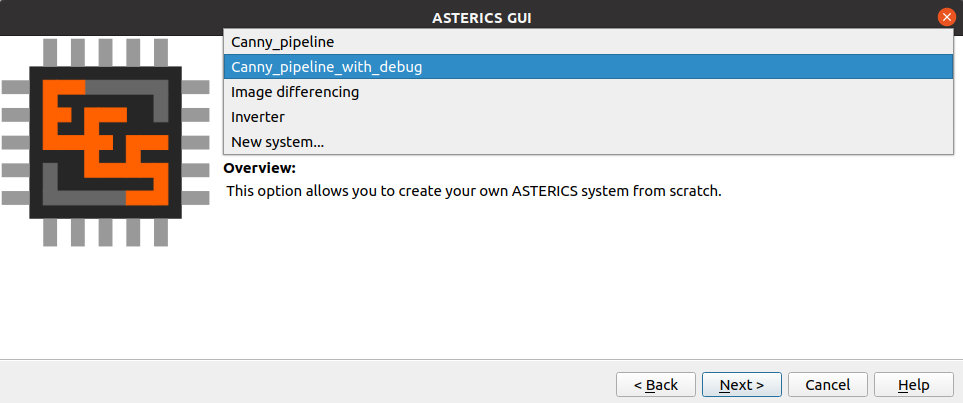
\includegraphics[width=\textwidth]{figs/gui/box}
			\caption{List on existing template}
			\label{fig:box}
		\end{minipage} 
		\hfill
		\begin{minipage}{0.47\textwidth}
			\centering
			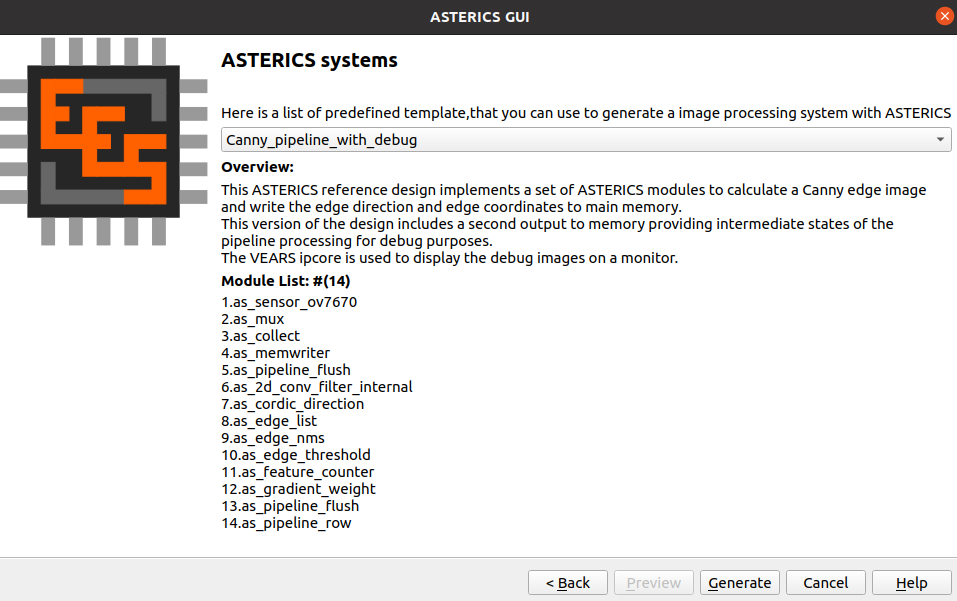
\includegraphics[width=\textwidth,]{figs/gui/exist}
			\caption{Description of an existing module}
			\label{fig:exist}
		\end{minipage}
	\end{figure}
	Compared to creating image processing systems from scratch, generating systems with template is faster. As it is shown in the figure \ref{fig:box}, there are already a few templates in \asterics. When a template is selected, a rough overview of the template's system is displayed, followed by a list of all modules involved in the chain. The system can then be created by clicking on the button \texttt{"Generate"}(see figure \ref{fig:exist}).
	
	\subsubsection{Use the generated Script}\label{subsub:06-05-generated-script}
	This section explains how to use the generated script.The generated script is located in the 4th view of Figure \ref{fig:GuiMainView} after clicking the "Generate" or "Finish" button of the wizard.  
	To save the script, you should click on the icon of the 4th view, which is the "Save As" button. You can manually customize the generated script again in your favorite editor after saving it. The script must be saved as Python file. Depending on whether the script was created from scratch or came from a demo system, the script will look different, especially when selecting the output products. Assuming that the script is saved under the name \texttt{"asterics-gen.py"}:
\begin{lstlisting}[style=AutomaticsPython, label=Code:06-05-demo-output-product, caption=Script: Demo system output product]

############### Automatics outputs ##############################

if len(sys.argv) < 3:
	print(
	(
		"Not enough parameters!\n"
		"Usage:\nasterics-gen.py build-target output-folder\n"
		"Valid build-targets: 'vivado', 'core'"
	)
 )
sys.exit()

# Build chain: Generate output products
# Write the outputs for the ASTERICS core

# Stores wether Automatics completed without errors or not
success = False

if sys.argv[1] == "vivado":
	success = chain.write_ip_core_xilinx(
	sys.argv[2] + "/ASTERICS", use_symlinks=True, force=True
	)
if success:
	# Create link to the VEARS IP-Core
	success = asterics.vears(sys.argv[2], use_symlinks=True, force=True)
elif sys.argv[1] == "core":
	success = chain.write_asterics_core(sys.argv[2], use_symlinks=True)
else:
	sys.exit("Not a valid build target!")
# On success, generate a system graph using dot
if success:
	chain.write_system_graph("asterics_system_graph")

# Report
if success:
	print("Automatics completed successfully!")
else:
	print("Automatics encountered errors:")
	asterics.list_errors()
\end{lstlisting}
	\begin{itemize}
		\item \textbf{Demo systems:}\\
			The script part representing the output products looks like in Listing \ref{Code:06-05-demo-output-product}. You can generate the output products using the following command line:
\begin{lstlisting}[style=shell]
$ python asterics-gen.py build-target output-folder
\end{lstlisting}
or 
\begin{lstlisting}[style=shell]
$ python3 asterics-gen.py build-target output-folder
\end{lstlisting}
			Where \textit{build-target} must be either \texttt{"vivado"} or \texttt{"core"}. With \texttt{"vivado"}, the \asterics system generator \automatics generates the source file for the described \asterics chain and packages them to an IP-Core using Xilinx Vivado. With \texttt{"core"}, \automatics generates only the \asterics chain source files to the the folder \textit{output-folder}. \textit{output-folder} is the name of the directory where the output products must be stored. For more information about the output product see \ref{ssec:02-output}.
		\item \textbf{Your own system:} \\
			For the systems you have built yourself, the script part representing the output products looks like in Listing \ref{Code:06-05-system-from-scratch-output-product}. All possible output products are listed. Depending on your application, you can generate only the necessary products. You only have to adjust the output folder \texttt{"destination\_dir"} and the path \texttt{"output\_file"} and then the script can be generated. After saving the generated script, run the command line to generate the output products:
\begin{lstlisting}[style=shell]
 $	python(3) asterics-gen.py
\end{lstlisting}
			
	\end{itemize}


\begin{lstlisting}[style=AutomaticsPython, label=Code:06-05-system-from-scratch-output-product, caption=Script: Output product of systems created with the wizard from scratch]
# Automatics output products 
# All possible output products are listed below and it is 
#			not necessary to generate all of them.
# vivado
chain.write_ip_core_xilinx(path='destination_dir', use_symlinks=True, 
							force=False, module_driver_dirs=False)
# Create link to the VEARS IP-Core
asterics.vears(path='destination_dir', use_symlinks=True, force=False)
# Core
chain.write_asterics_core(path='destination_dir', use_symlinks=True, 
							force=False, module_driver_dirs=False)
# System
chain.write_system(path='destination_dir', use_symlinks=True, 
	force=False, module_driver_dirs=False, add_vears=False)
# SVG graph
chain.write_system_graph(out_file='output_file', show_toplevels=False, 
						show_auto_inst=False, show_ports=False, 
						show_unconnected=False, show_line_buffers=False)
\end{lstlisting}
\begin{figure}[h]
	\centering
	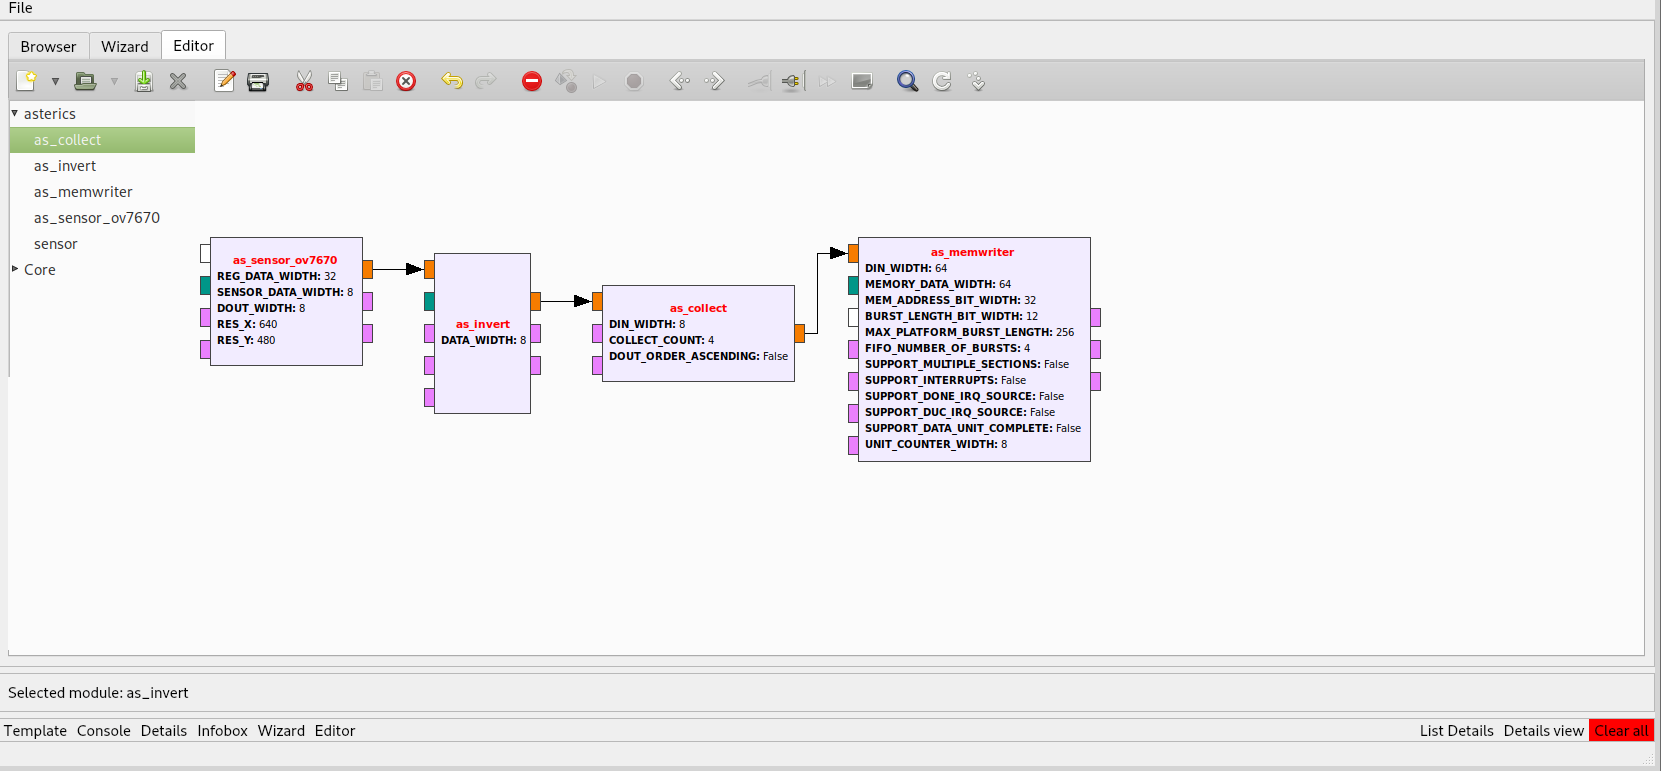
\includegraphics[width=\textwidth]{figs/gui/editor}
	\caption{Inverter system with editor.}
	\label{fig:editor}
\end{figure}
	\subsection{Editor}\label{sec:06-05-editor}
		The editor is currently under development and it should make the creation of image processing chains even easier and faster. It should not only be possible to create simple image processing chains, but also complex ones and the representation of systems should also be possible graphically. Figure \ref{fig:editor} shows an inverter system with the current version of the editor.
	\newpage	
		
		
